%%#################################################################
%% CHAPTER 2
%%#################################################################
\chapter{History and Theoretical Foundations}
\label{cha:SoA}

\begin{ChapAbstract}
Where we present the historical and theoretical context for this thesis. We briefly present the sequence of events which resulted in this thread of research, and present the main definitions and base concepts needed to understand this work.
\end{ChapAbstract}


\section{A Historical Overview}
The field of Artificial Intelligence\footnote{As one would expect, only part of the last fifty years are addressed in these brief paragraphs, in particular those that are relevant for this thread of research in Artificial Intelligence.} (AI) has grown in both depth and breadth since its very name was coined at the 1956 Dartmouth College meeting\cite{dartmouth}. If, in those early days, AI was hardly considered a science, it didn't take long for formal methods of research and development to appear. The area soon became richer in its various approaches to the challenge of providing computers with methodologies similar to those used by humans to solve problems.

From the several approaches that followed the Dartmouth meeting regarding knowledge representation, one was related with the use of logical formulas to express knowledge. It was around 1960 that John McCarthy first expressed the advantages of such approach\cite{commonSense}:

\begin{quotation}
``Expressing information in declarative sentences is far more modular than expressing it in segments of computer programs or in tables. Sentences can be true in a much wider context than specific programs can be used. The supplier of a fact does not have to understand much about how the receiver functions or how or whether the receiver will use it. The same fact can be used for many purposes, because the logical consequences of collections of facts can be available.''
\end{quotation}

Other authors defended this orientation, namely Patrick Hayes\cite{philoProblems}, Nils J. Nilsson\cite{logicAI} and Drew McDermott\cite{critique}, which ended up originating two main threads of research, initially very distinct but later converging on the same line of work.

The first of these was Logic Programming (LP). Logic Programming, the application of automatic methods of deduction combined with logic-based knowledge representation, was started by Alain Colmerauer \cite{prologReport} and Robert Kowalski\cite{logicAlgorithmControl,kowalskiPredicate}, and introduced in Computer Science the idea of a declarative logical approach to programming, as opposed to a procedural one. This new programming paradigm was summarized by Robert Kowalski in \cite{logicAlgorithmControl}, and ended up providing a fast proliferation of the logic-based approach to AI, as researchers now had a way to implement and test their theories. Logic programming eventually came to life under the Prolog\footnote{Prolog is an abbreviation of \emph{PROgrammation en LOGique}, name suggested by Philippe Roussel\cite{birthProlog}.} language in 1972 by the hand of Colmerauer and Kowalski, which not only did it demonstrate that Prolog was a practical language as it also helped disseminate it worldwide. Nowadays several Prolog distributions exist, making LP a relevant paradigm in Computer Science.

During the same years, other researchers were delving into the problems of performing commonsense reasoning in AI. John McCarthy was perhaps the first person to consider these issues\cite{commonSense} and later, together with Patrick Hayes\cite{philoProblems}, introduced the Frame Problem. The Frame Problem deals with the representation of things that do not change in a given situation, when a certain event occurs. This frame problem was precisely the kind of problem to be addressed by nonmonotonic reasoning, the fact that monotonic classical logic \emph{per se} does not deal correctly with changing worlds. The term \emph{nonmonotonic reasoning} is probably attributed to Marvin Minsky in \cite{nmrTermIntroduction}, where he also summarizes his critique to classical logic. 

Both threads of research continued to evolve rather separated from each other, until 1986. In 1986, at the Workshop on the Foundations of Deductive Databases and Logic Programming, a major milestone was reached with the Stratified Semantics -- it is a semantics of interest for the LP community, but its underlying principles are more closely related to those of NMR. It was a milestone precisely because this and the group of semantics that followed, left the operational concerns of classical LP behind and were more concerned with their suitability for practical applications and NMR. 

During the following years, several different semantics appeared and important relations between them and NMR were discovered. Of particular interest to this work are the following moments:

\begin{itemize}
	\item 1988, introduction of the Stable Models Semantics\cite{smMain};
	\item 1991, introduction of the Well-Founded Semantics\cite{wfsMain};
	\item 2004, introduction of the Revised Stable Models Semantics\cite{ampMSc, rsmEpia}.
\end{itemize}

These semantics set the grounds for this work and constitute the last steps in the thread of research we have described so far.

In the remainder of the chapter, we'll introduce the theoretical notions required for the understanding of this work, as well as the semantics it is based on. We end up with a motivation for the \rwfs, the main theme of this thesis.


\section{Language of Logic Programs and Other Common Definitions}
We now present the theoretical context for this thesis by showing several basic definitions that will be used throughout this work.

We start by defining an alfabet\footnote{The definitions in this section are borrowed and extended from \cite{aparasPhD,jjaPhD,milkBook}.} $\cal{A}$ over a language $\cal{L}$, which is a finite or countably infinite disjoint set of constants, predicate symbols with associated arity, function symbols with associated arity, as well as a countably infinite set of distinguished variables.


\begin{definition}[Term]
A term over $\cal{A}$ is defined as one of the following:
\begin{itemize}
	\item A variable, which we'll normally write as $X$, in uppercase;
	\item A constant, which we'll normally write as $x$, in lowercase;
	\item A function symbol $f(t_{1},\ldots,t_{n})$ with $t_{1},\ldots,t_{n}$ being terms;
\end{itemize}
A term is said to be ground if it doesn't contain variables.
\end{definition}

\begin{definition}[Atom]
An atom is either a term or an expression $p(t_{1},\ldots,t_{n})$, where $p$ is a predicate symbol and $t_{1},\ldots,t_{n}$ are terms. An atom is ground if all its terms are grounded.
\end{definition}

\begin{definition}[Herbrand base]
The set of all ground atoms is called the Herbrand base and is represented as $\cal{H}$.
\end{definition}

\begin{definition}[Literal]
A literal is either an atom $A$ or its default negation $\sim A$. 
We will use the symbol $\sim$ to refer to the implicit negation, or default negation. Hence, literals can also be called positive literals or default (negative) literals, whether they are respectively non-negated literals or negated literals.
A literal is said to be ground if it doesn't contain any variable.
\end{definition}

\begin{definition}[Rule]
A rule is a clause over $\cal{A}$ in the form
\begin{align*}
H\leftarrow A_{1},\ldots,A_{n}
\end{align*}
where $H$ is a positive literal and $\{A_{1},\ldots,A_{n}\}$ are positive or negative literals. $H$ is called the head of the rule while $\{A_{1},\ldots,A_{n}\}$ constitutes the body of the rule. If a rule doesn't contain a body it is called a fact and is represented as 
\begin{align*}
H\leftarrow 
\end{align*}
\end{definition}

\begin{definition}[Heads and Bodies of rules]
Regarding rules we define the functions $head(r)$ and $body(r)$ which, for any rule $r$ respectively give as a result its head and its body.

Given a set of rules $S$, the functions $heads(S)$ and $bodies(S)$ respectively give as a result the set of all heads of all rules of $S$ and the set of all bodies of all rules of $S$.
\end{definition}


From these definitions we can now specify what we mean by a \DefP and a \NLP.

\begin{definition}[\DefP]
A \defp (DP) $P$ is a countable set of rules, such that their bodies only include positive literals.
\end{definition}

\begin{definition}[\NLP]
A \nlp (NLP) $P$ is a countable set of rules.
\end{definition}

The transition from NLPs, which are only syntactic descriptions of some world or situation, to the meaning they have is done through the following definitions regarding interpretations and models.


\begin{definition}[Two valued Interpretation]
A \twovi $I$ of a NLP $P$ is any subset of the Herbrand base $\cal{H}$ of $P$, and can be viewed as the set
\begin{align*}
I=\cal{T}\cup\sim \cal{F}
\end{align*}
where $\cal{T}\subseteq I$ is the set of ground atoms true in $I$ and $\cal{F}=\cal{H}\setminus \cal{T}$ is the set of ground atoms false in $I$.
\end{definition}

\begin{definition}[Three valued Interpretation]
\label{def:threeVI}
A \threevi $I$ of a NLP $P$ is a set
\begin{align*}
I=\cal{T}\cup\sim \cal{F}
\end{align*}
where $\cal{T}$ and $\cal{F}$ are disjoint sets of the Herbrand base $\cal{H}$ of $P$ and $\cal{T}$ is the set of ground atoms true in $I$ and $\cal{F}$ is the set of ground atoms false in $I$. The truth value of the remaining ground atoms is undefined.
\end{definition}

For the sake of simplicity, we'll often refer to two-valued interpretations only by including the set of atoms that are true ($\cal{T}$), and \threevi by including the set of atoms which are true, and those which are true or undefined as a tuple $\langle\cal{T},\cal{TU}\rangle$.

Interpretations can be viewed as \emph{possible worlds} of a program $P$, as it is discussed by Przymusinska and Przymusinski\cite{semanticIssues} which correspond to possible states of knowledge regarding program $P$. Three valued interpretations account for the possibility of not knowing everything about the world, and being able to represent the things known to neither be definitely true nor definitely false.

\begin{definition}[Satisfaction]
Given an interpretation $I$ (two valued or three valued) and a NLP $P$ we say that:
\begin{itemize}
	\item $I$ satisfies a literal $X$, denoted by $I\models X$, iff $X\in I$;
	\item $I$ satisfies the conjunction $X_{1},\ldots,X_{n}$, denoted by $I\models \{X_{1},\ldots,X_{n}\}$, iff $I\models X_{1},\ldots,I\models X_{n}$;
	\item $I$ satisfies the rule $H\leftarrow X_{1},\ldots,X_{n}$, denoted by $I\models (X_{1},\ldots,X_{n})$, iff whenever the conjunction $X_{1},\ldots,X_{n}$ is satisfied by $I$, then $H$ is also satisfied by $I$.
\end{itemize}
\end{definition}



\section{Stable Models Semantics and the Well-Founded Semantics}
Gelfond and Lifschitz introduced the \SMs Semantics (SMs) in 1988\cite{smMain}, a semantics which would end up becoming one of the most important in the field of logic programming. 

The main idea behind the \sms comes from the field of \nmr, following the sequence of events detailed in the previous section. Its intuition is that if we assume some literals as true and others as false, those assumptions should be corroborated by the semantics of definite programs\cite{predicateProgramming}. If they are, then they form a stable model. This semantics makes use of an operator that, given a \twovi $I$, transforms the NLP into a definite program (DP), in order to calculate its least model.

\begin{definition}[\GFo $\Gamma$]
Let $P$ be a NLP and $I$ a \twovi. The GL-transformation of $P$ modulo $I$ is the program $\frac{P}{I}$ obtained from $P$ by performing the following operations:

\begin{itemize}
	\item Remove from $P$ all rules containing a default literal $\sim X$, such that $X\in I$;
	\item Remove from the remaining rules all the other default literals.
\end{itemize}

Since $\frac{P}{I}$ is a DP, it has a unique least model $J$.

Let $\Gamma_{P}(I)=J$.
\end{definition}



\begin{definition}[\SMs Semantics]
A \twovi $I$ of a NLP $P$ is a Stable Model of $P$ iff $\Gamma_{P}(I)=I$.

A ground atom $X$ of $P$ is true under the \sms semantics iff $X$ belongs to all stable models of $P$.

We represent a \sm $M$ of a NLP $P$ as $SM_{P}(M)$.
\end{definition}

It was soon discovered\cite{bidoit,gelfondStratified} that the \sms are closely related to \nmr formalisms, namely Reiter's default extensions\cite{reiterDefault} and Moore's autoepistemic extensions\cite{mooreAutoepistemic}. This close relation helped bring the fields of \NMR and Logic Programming closer, by providing LP with \nmr formalisms and NMR with a practical vehicle of experimentation and research.

Besides this important relation, the SMs ended up being defined for the extended class of logic programs, i.e., logic programs with classical negation. The resulting semantics, the Answer Set Semantics\cite{answerSets} is one of the most used in Multiagent Systems and Artificial Intelligence applications where the knowledge representation approach based on logic.

The SMs have, however, some important drawbacks. First of all, the \sms semantics is not always consistent, which means that some programs have no semantics at all. Consider, for example 
\begin{align*}
P=\{a&\leftarrow\sim a\}
\end{align*}

$\Gamma_{P}(\{a\})=\{\}$ but $\Gamma_{P}(\{\})=\{a\}$, which means $P$ has no semantics whatsoever, because there is no single interpretation $I\subseteq{\cal{H}}_{P}$ such that $\Gamma_ {P}(I)=I$. Additionally, the SMs also lack the properties of Cumulativity (the addition of lemmas from a model to the original program doesn't alter the semantics) and Relevancy (the possibility of implementing a top-down query-driven proof-procedure), and its computation, even brave-reasoning, is NP-Complete\cite{npComputation}.

Three years passed since the introduction of the SMs until Alan van Gelder along with Kenneth Ross and John Schlipf proposed\cite{wfsMain} the Well-Founded Semantics (WFS). The WFS overcomes all the problems described before and still maintains a strong relation with NMR formalisms. It is more expressive than the \sms semantics as it uses three-valued interpretations but is also a lot more skeptical, attributing the value of undefined to all those literals which are not undoubtfully true or false (or depend on ones who are, in turn, undefined), or lack classical support.

Several definitions of the \wfs exist in the literature. For this work, we'll make use of the one defined by Baral and Subrahmanian\cite{wfsDualities}, which is most closely related with our approach to the subject of this thesis.

\begin{definition}[\BSo $\Gamma^{2}$]
Let $P$ be a NLP and $I$ an two-valued interpretation. The \BSo $\Gamma^{2}$ is defined as being two applications of the \GFo $\Gamma$:
\begin{align*}
\Gamma_{P}^{2}(I) = \Gamma_{P}(\Gamma_{P}(I))
\end{align*}
\end{definition}

\begin{definition}[\WFS]
Let $P$ be a NLP. The \WFS of program $P$ is the tuple $\left\langle \cal{T},\cal{TU} \right\rangle$, with $\cal{T}$ corresponding to the true literals according to the semantics and $\cal{TU}$ being the true or undefined literals according to the semantics.

The $\cal{T}$ set can be calculated as being the least fixed point of $\Gamma_{P}^{2}$ starting with the empty interpretation, i.e., $\cal{T}=$$\Gamma_{P}^{2\text{ }\uparrow \omega}(\{\})$, with $\omega$ being the least limit ordinal.

The $\cal{TU}$ set can be calculated as being the next iteration of $\Gamma_{P}$, starting from the $\cal{T}$ set, i.e., $\cal{TU}=$$\Gamma_{P}(\cal{T})$.

We will refer to the \wfm $M$ of any NLP $P$ as $WFM_{P}(M)=\langle\cal{T},\cal{TU}\rangle$. The $\cal{T}$ set of the WFM will be referred to as \tWFM and the set $\cal{TU}$ of the WFM will be referred to as \tuWFM.
\end{definition}

The \wfs has all the properties the \sms miss, namely cumulativity, relevancy and existence. Furthermore, it ensures uniqueness of model, a property desirable for the \wfs. Its \wfm is computable in polynomial time and several WFS implementations (\cite{xsbSite,xsbArticle,branchBound,alternatingFixpoint}) have been studied and exist nowadays. Moreover, several important relations exist between the \wfs and \nmr formalisms\cite{wfsDualities,wfsGeneralized}, as well as between the \wfs and the \sms semantics\cite{wfsCoincides,wfsRelation}. Additionally, the WFS was later expanded to its explicit\cite{jjaPhD,wfsxArticle}, paraconsistent\cite{paraconsistentArticle} and disjunctive\cite{alcantaraPhD} counterparts. It falls out of the scope of this thesis to analyse and comment on these relations; the key subject here is that the WFS ended up being heavily studied.

During the last decades, these two semantics were extensively used and studied for \nmr and \kr. The \sms semantics on one side, when researchers needed a two-valued semantics, capable of representing several possible worlds as models of a program; and the \wfs on the other side, when researchers were willing to sacrifice the expressiveness of having multiple two-valued models in order to have a three-valued skeptical and sure-footed semantics.


\section{Enter the \RSMs}
The drawbacks of the \sms semantics, described in the previous section, are dealt with in the \wfs but they aren't actually \emph{solved}. Only in 2004 Pinto and Moniz Pereira proposed\cite{rsmItaly} a way of solving the problems of the \sms and have been studying\cite{ampMSc,rsmEpia,rsmItaly} its aspects ever since.

The Revised Stable Models (rSMs) is a semantics for NLPs which applies the principle of \RAA (RAA) to solve the main problems of the \sms semantics, namely inconsistency, cumulativity and relevancy. Inconsistency in SMs, as it was shown by François Fages\cite{fages}, comes from the existence of \olons (OLONs) in the program such as
\begin{align*}
P=\{a\leftarrow\sim a\}
\end{align*}

François Fages goes on explaining that not only OLONs are the source of the problem for inconsistency, but also \icons (ICONs), as in the case of:
\begin{align*}
P=\{& p(X)\leftarrow p(s(X))\\
& p(X)\leftarrow\sim p(s(X))\}
\end{align*}

In a nutshell, according to the principle of \raa if a certain hypothesis leads to a contradiction, it should be withdrawn. In the first case, by assuming $\sim a$ as true, this assumption will eventually lead us to conclude $a$, a contradiction. Therefore $\sim a$ cannot be concluded, so $a$ should be. In the second case, if we assume $\sim p(X)$ then the bodies of both rules should be false, which is impossible since they are logical oppositions. Therefore, $p(X)$ must be true, as $\sim p(X)$ will never be.

\RSMs are in everything similar to the \sms, only changing the way the semantics deals with OLONs and ICONs -- it solves them using RAA reasoning, given that the conclusions derived from this resolution keep consistent with the rest of the program. This results in an extension to the \sms semantics, which solves all the problems detailed previously.


\begin{definition}[Sustainable Set\cite{ampMSc,rsmEpia}]
\label{def:sustainable}
As a shorthand notation only for this definition, let $WFM(P)$ denote the positive atoms of the Well-Founded Model of $P$, that is WFM(P) is the least fixed point of operator $\Gamma_{p}^{2}$\cite{wfsDualities}, i.e., $\Gamma_{p}$ applied twice. Intuitively, we say a set $S$ is sustainable in $P$ if and only if any atom $A$ in $S$ does no go against the well-founded consequences of the remaining atoms in $S$ whenever $S\setminus\{A\}$ itself is a sustainable set. The empty set by definition is sustainable. ``Not going against'' means that atom $A$ cannot be false ($A$ is true or undefined) in the well-founded model of $P\cup S\setminus\{A\}$, i.e., it belongs to set $\Gamma_{P\cup S\setminus\{A\}}(WFM(P\cup S\setminus\{A\}))$

Formally we say $S$ is sustainable if and only if:

\begin{center}
\begin{math}
\forall_{A\in S}, S\setminus\{A\}\ is\ sustainable\Rightarrow A\in \Gamma_{P\cup
S\setminus\{A\}}\left(WFM\left(P\cup S\setminus\{A\}\right)\right)
\end{math}
\end{center}

If $S$ is empty the condition is trivially true.
\end{definition}


\begin{definition}[Revised \SMs and Semantics\cite{ampMSc,rsmEpia}]
\label{def:rsms}
Let $RAA_{P}(M)\equiv M\setminus\Gamma_{P}(M)$. $M$ is a Revised Stable Model of an Normal \LP $P$, if and
only if:
\begin{itemize}
\item $M$ is a minimal classical model, with ``$\sim$'' interpreted as classical
negation;
\item $\exists_{\alpha\ge 2}$ such that $\Gamma_{P}^{\alpha}(M)\supseteq
RAA_{P}(M)$
\item $RAA_{P}(M)$ is sustainable.
\end{itemize}

The Revised \SMs semantics is the intersection of its models, just as in the \sms semantics.

We represent a \rsm $M$ of a NLP $P$ as $rSM_{P}(M)$.
\end{definition}

As it was proven in \cite{ampMSc}, the \rsms enjoy not only the existence of model property, therefore loosing the inconsistency the SMs had, as well as the properties of cumulativity and relevancy. They also served as a preliminary proof that the principle of \raa could be used as an additional form of support, which is a very important result for the context of this thesis.


\section{The Next Step}
This semantics and the additional notion of support it employs, somewhat change the map of \kr and \nmr semantics we have detailed so far.


\begin{figure}[htbp]
	\centering
		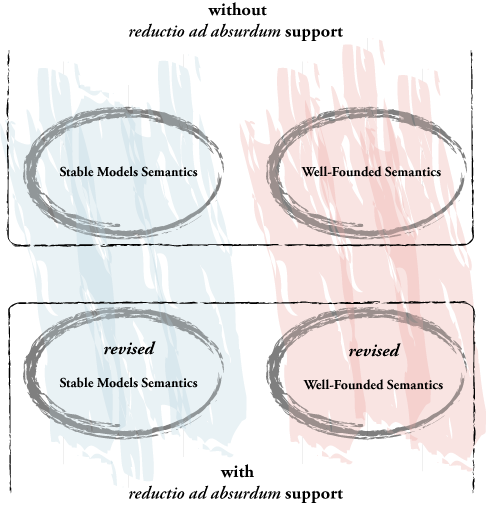
\includegraphics[width=0.55\textwidth]{Chap2/transitions.png}
	\caption{\footnotesize Map of transition and relations between the existing semantics for \nlps. Note that in the blue area, on the left, we have two-valued semantics while in the red area, on the right, we have the three-valued semantics. Additionally, the bottom of the figure represents semantics with RAA support, while the top of the figure represents those without RAA support.}
	\label{fig:transitions}
\end{figure}



The top level of figure \ref{fig:transitions} represents the current state of the art in semantics for \nlps \emph{without} RAA support. The \sms represent a flexible two-valued semantics, capable of representing several possible worlds in its various models. The \wfs represents a single three-valued view of a \nlp, enjoying several important properties but being too skeptical in its conclusions. The bottom level of the figure represents the corresponding semantics employing the principle of \raa as an additional form of support. The \rsms solve all the problems the \sms had, becoming a semantics as flexible as the SMs, with some of the properties the WFS had. All it's missing to define is the \RWFS, a three-valued counterpart of the rSMs and the next transition point from the WFS, when using the RAA notion of support.

In the next chapter we'll discuss the motivation for the definition of a rWFS, and continue providing its declarative definition. We'll then discuss the properties it enjoys when compared with the WFS and present some examples of its calculation.
